\RequirePackage{fix-cm}
\documentclass[twocolumn]{svjour3}          %
\smartqed  %
\usepackage{times}
\usepackage{epsfig}
\usepackage{graphicx}
\usepackage{amsmath}
\usepackage{amssymb}
\usepackage{adjustbox}
\usepackage{mathtools}
\usepackage{xspace}
\usepackage{cite}
\usepackage{xcolor}
\definecolor{citecolor}{HTML}{0071bc}
\usepackage[pagebackref=true,breaklinks=true,letterpaper=true,colorlinks,citecolor=citecolor,bookmarks=false]{hyperref}

\DeclarePairedDelimiter{\floor}{\lfloor}{\rfloor}
\newcommand{\eg}{\textit{e.g.}}
\newcommand{\ie}{\textit{i.e.}}
\newcommand{\set}[1]{\{{#1}\}}
\newcommand{\D}{\mathcal{D}}
\newcommand{\KL}[2]{\mathop{KL}({\textstyle #1}\,\|\,{{\textstyle
      #2}})}
\def\etal{{\em et al.\/}\,}
\def\argmax{\mathop{\rm argmax}}
\def\argmin{\mathop{\rm argmin}}
\def\tr{\mathsf{tr}}
\def\diag{\mathsf{diag}}
\newcommand{\indep}{{\;\bot\!\!\!\!\!\!\bot\;}}
\newcommand\todo[1]{\textcolor{red}{[TODO: #1]}}
\newcommand\new[1]{\textcolor{blue}{#1}}
\newcommand{\prgan}{\textsc{PrGAN}\xspace}
\newcommand{\prgans}{\textsc{PrGANs}\xspace}
\newcommand{\norm}[1]{\left\lVert#1\right\rVert}

\begin{document}

\title{Inferring 3D Shapes from Image Collections using Adversarial Networks%
}


\author{Matheus Gadelha \and
        Aartika Rai  \and
        Subhransu Maji  \and
        Rui Wang
}


\institute{Matheus Gadelha, Aartika Rai, Subhransu Maji, Rui Wang \at
  College of Information and Computer Sciences, University
  of Massachusetts Amherst,   140 Governors Dr, Amherst, MA 01003, USA\\
  \email{\{mgadelha, aartikarai, smaji, ruiwang\}@cs.umass.edu}           %
}

\date{Received: date / Accepted: date}


\maketitle


\begin{abstract}
We investigate the problem of learning a probabilistic distribution over
three-dimensional shapes given two-dimensional views of multiple
objects taken from unknown viewpoints.
Our approach called \emph{projective generative adversarial network}
(\prgan) trains a deep generative model of 3D shapes whose projections
(or renderings) matches the distribution of the provided 2D views.
The addition of a \emph{differentiable projection
module} allows us to infer the underlying 3D shape distribution without
access to any explicit 3D or viewpoint annotation during the learning
phase. 
We show that our approach produces 3D shapes of comparable
quality to GANs trained directly on 3D data. %
Experiments also show that the
disentangled representation of 2D shapes into geometry and viewpoint
leads to a good generative model of 2D shapes.
The key advantage of our model is that it estimates 3D shape, viewpoint, and generates novel
views from an input image in a completely unsupervised manner.
We further investigate how the generative models can be improved
if additional information such as depth, viewpoint or part
segmentations is available at training time.
To this end, we present new differentiable projection operators that can be
used to learn better 3D generative models.
Our experiments show that \prgan can successfully leverage extra visual cues
to create more diverse and accurate shapes.
\end{abstract}

\section{Introduction}\label{xs:intro}

\begin{figure}[t]
\centering
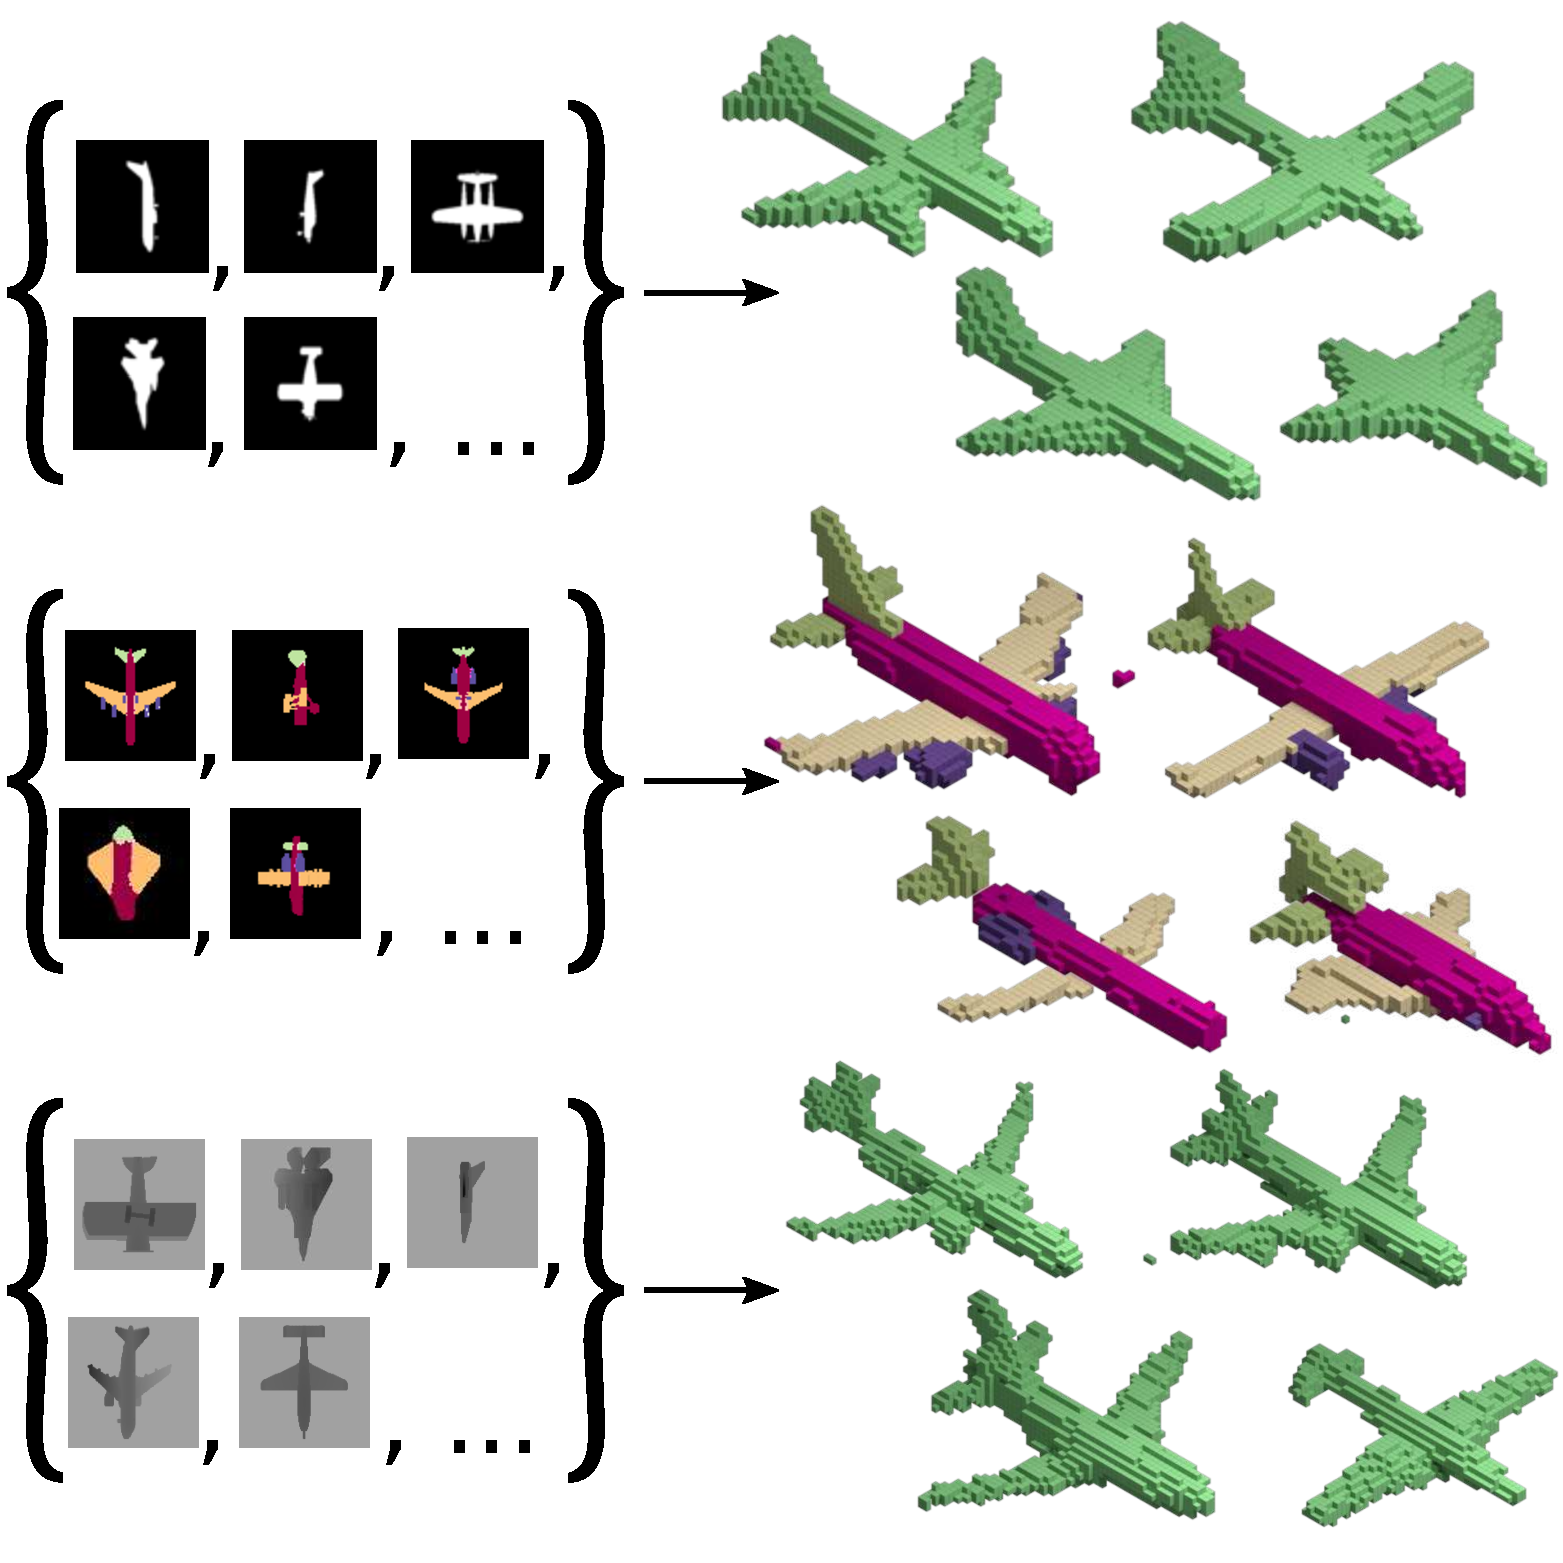
\includegraphics[width=1.0\linewidth]{fig/visabstract.pdf}
\caption{\label{f:problem} Our algorithm infers a generative model of
  the underlying 3D shapes given a collection of unlabeled images rendered as
  silhouettes, semantic segmentations or depth maps. 
	To the left, images representing the input dataset.
	To the right, shapes generated by the generative model trained with those images.}
\vspace{-12pt}
\end{figure}


The ability to infer 3D shapes of objects from their 2D views is one
of the central challenges in computer vision.
For example, when presented with a catalogue of airplane silhouettes
as shown in the top of Figure~\ref{f:problem}, one can mentally infer
their 3D shapes by simultaneously reasoning about the shape and
viewpoint variability.
In this work, we investigate the problem of learning a generative
model of 3D shapes from a collection of images of an unknown set of
objects within a category taken from an unknown set of views.
The images can be thought of as generalized projections of 3D shapes
into a 2D space in the form of silhouettes, depth maps,
or even part segmentations.
The problem is challenging as one is not provided with the information
about which object instance was used to generate each image, the viewpoint from
which each image was taken, the parameterization of the underlying shape
distribution, or even the number of underlying instances.
Hence, traditional techniques based on structure
from motion~\cite{hartley2003multiple,blanz1999morphable} or visual
hulls~\cite{laurentini1994visual}, cannot be directly applied.


We use the framework of generative adversarial
networks (GANs)~\cite{goodfellow2014generative} and augment the 3D shape
generator with a \emph{projection module}, as illustrated in Figure~\ref{fig:prgan-arch}.
The generator produces 3D shapes, the projection module
renders the shape from viewpoint sampled from a viewpoint distribution,
and the adversarial network discriminates real images from generated ones.
The projection module is a \emph{differentiable renderer} that allows us to map 3D
shapes to 2D images, as well as back-propagate the gradients of 2D
images to 3D shapes.
Once trained, the model can be used to infer 3D shape distributions
from a collection of images (Figure~\ref{f:problem} shows some samples
drawn from the generator), and to infer depth or viewpoint from a single
image, without using any 3D or viewpoint information during learning.
We call our approach \emph{projective generative adversarial network}
~(\prgan).








While there are several ways of rendering a 3D shape, we begin with a 
silhouette representation.
The motivation is that silhouettes can be easily
extracted when objects are photographed against clear backgrounds, such
as in catalogue images, but nevertheless they contain rich shape information.
Real-world images can also be used by removing background and converting them to
binary images. 
Our generative 3D model represents shapes using a voxel representation that indicates
the occupancy of a volume in a fixed-resolution 3D grid.
Our projection module is a feed-forward operator that
renders the volume as an image.
The feed-forward operator is differentiable, providing
the ability to adjust the 3D volume based on projections. 
Finally, we assume that the distribution over viewpoints
is known (assumed to be uniform in our experiments, but it could be any
distribution).

We then extend our analysis first presented in our earlier
work~\cite{prgan} by incorporating recent advances in training GANs and
designing projection modules to incorporate richer supervision.
The latter includes the availability of viewpoint information for
each image, depth maps instead of silhouettes, or semantic
segmentations such as part labels during learning.
Such supervision is easier to collect than acquiring full 3D scans of
objects.
For example, one can use a generic object viewpoint
estimator~\cite{su2015render} as weak supervision for our problem.
Similarly, semantic parts can be labeled on images directly and
already exist for many object categories such as airplanes, birds,
faces, and people.
We show that such information can be used to improve 3D reconstruction
by using an appropriate projection module.

To summarize our main contributions are as follows: (i) we propose
\prgan, a framework to learn probabilistic distributions over 3D
shapes from a collection of 2D views of objects. We demonstrate its
effectiveness on learning shape categories
such as chairs, airplanes, and cars sampled from online shape
repositories~\cite{chang2015shapenet,wu20153d}. 
The results are reasonable even when views from multiple categories
are combined; (ii) \prgan generates 3D shapes of comparable quality to GANs trained
directly on 3D data~\cite{wu2016learning};
(iii) The learned 3D representation can be used for unsupervised
estimation of 3D shape and viewpoint given a novel 2D shape, 
and for interpolation between two different shapes, (iv) Incorporating
additional cues as weak supervision improves the 3D shapes
reconstructions in our framework.



\section{Related Work}
A number of approaches have studied 3D shape recognition and generation using uniform 3D voxel grids~\cite{choy20163d,wu20153d,Huang:PCL,voxnet,BrockLRW16,3dgan}.
However, uniform grids have poor scalability and require large memory footprint, hence existing networks built upon them often operate on a relatively low-resolution grid. 
Several recent works address this issue through multiscale and sparse representations~\cite{Riegler2017CVPR,tatarchenko2017octree,ocnn,hie3dcnn,splatnet,graham17sparse} at the expense of additional book keeping. 
Still, voxel-based methods generally incur high processing cost, and are not well suited for modeling fine surface details. 
Moreover, it's not clear how to incorporate certain geometric attributes, like surface normals, into voxel representation, since these attributes do not exist in the interior of the shape.




Multiview methods~\cite{mvcnn,qi2016volumetric,Soltani17,LunGKMW17,kalogerakis20173d} represent a 3D shape as images rendered from different viewpoints. 
These methods use efficient convolutional and pooling operations and leverage deep networks pretrained on large labeled image datasets.
However, they are not optimal for general shapes with complex interior structures due to self occlusions.
Nonetheless since most models on existing shape repositories are described well by their exterior surface, view-based approaches have been adapted
for shape classification and segmentation tasks. 
Recently they have also been used for generation where a set of depth and normal maps from different viewpoints are inferred using image-based networks, and have been successfully used for image to shape generation tasks~\cite{LunGKMW17,lin2018learning}.
However such approaches requires subsequent processing to resolve view inconsistencies and outliers which is a challenging task.

Previous work has also studied extensions of ConvNets to mesh surfaces such as spectral CNNs~\cite{bruna:spectral,Yi:SyncSpec:2017}, geodesic CNNs~\cite{masci:gcnn}, or anisotropic CNNs~\cite{Boscaini2016LearningSC}. They have shown success for local correspondence and matching tasks. However, some of these methods are constrained on manifold surfaces, and generally it's unclear how well they perform on shape generation tasks.
A recent work in~\cite{SimonovskyK17} generalized the convolution operator from regular grid to arbitrary graphs while avoiding the spectral domain, allowing graphs of varying size and connectivity. 

Another branch of recent works focused on processing shapes represented as point clouds. One example is PointNet~\cite{pointnet,pointnet2}, that directly consumes point clouds as input. The main idea is to first process each point identically and independently, then leverage a symmetric function (max pooling) to aggregate information from all points. The use of max pooling preserves the permutation invariance of a point set, and the approach is quite effective for shape classification and segmentation tasks. Similarly, KD-net~\cite{Klokov_2017_ICCV} operates directly on point cloud shapes. It spatially partitions a point cloud using a kd-tree, and imposes a feed-forward network on top of the tree structure. This approach is scalable, memory efficient, achieves competitive performance on shape recognition tasks. 
While successful as encoders, it hasn't been shown how these networks can be employed as decoders for shape generation tasks.



Generating shapes as a collection of points without intermediate modeling of view-based depth maps has been relatively unexplored in the literature.
The difficulty stems from the lack of scalable approaches for generating sets.
Two recent works are in this direction.
Fan et al.~\cite{fan2016point} train a neural network to generate point clouds from a single image by minimizing Earth Mover's Distance (EMD) or Chamfer distance (CD) between the generated points and the model points. These distances are order invariant and hence can operate directly on point sets. 
This approach uses a two-branched decoder, one branch is built with 2D transposed convolutions and the other one is composed by fully connected layers.
On the other hand, our approach uses a simpler and shallower decoder built as a composition of 1D deconvolutions that operate at multiple scales.
This representation improves information flow across scales, which leads to higher quality generated shapes. 
Moreover, we use permutation invariant losses along with regularization of latent variables to build a model similar to a variational autoencoder~\cite{vae}
that can be used to sample shapes from gaussian noise.
Another work in~\cite{Gadhela:2017:3DSG} learns a distribution over shape coefficients using a learned basis for a given category using a generative adversarial network~\cite{goodfellow2014generative}. 
However, in this approach, the underlying generative model assumes a linear shape basis, which produces less detailed surfaces. 
The improved scalability of our method allows generating shapes with more points and more accurate geometric details in comparison to previous work.




Our tree network builds on the ideas of multiscale~\cite{he2014spatial,lin2016fpn}, mutligrid~\cite{multigrid} and dilated~\cite{yu2015multi} or atrous filters~\cite{dutilleux1990implementation,chen2016deeplab} effective for a number of image recognition tasks. 
They allow larger receptive fields during convolutions with a modest increase in the number of parameters.
In particular Ke et al.~\cite{multigrid} showed that communication across multiresolutions of an image throughout the network leads to improved convergence and better accuracy on a variety of tasks.
Our approach provides an efficient way of building multigrid-like representations for 3D point clouds.



\section{Method}\label{pca:method}

\begin{figure}
\centering
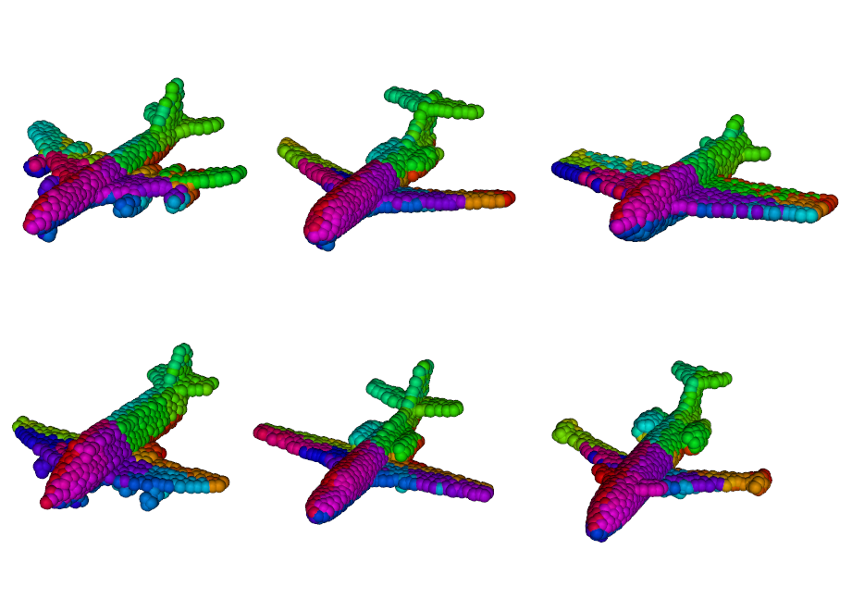
\includegraphics[width=0.49\linewidth]{PCAGAN/images/airplanes_sorting_new2.png}

\includegraphics[height=1.4in]{PCAGAN/images/vline.png}
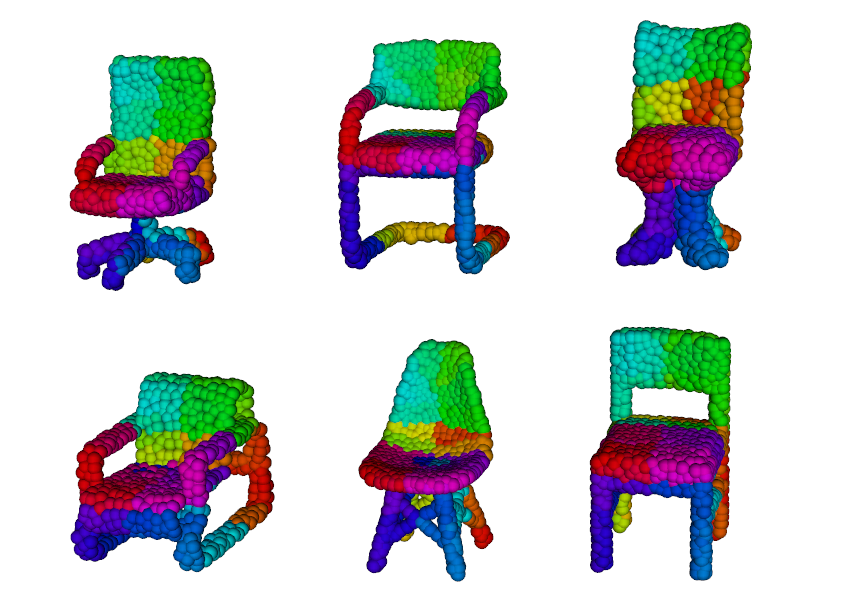
\includegraphics[width=0.49\linewidth]{PCAGAN/images/chairs_sorting.png}
\vspace{-12pt}
\caption{\small \label{fig:point_sorting} Visualization of spatially partitioned points for six training shapes from each category. Every point is colored by its index in the sorted order. This shows that the kd-tree sorting leads to reasonably good correspondences between points across all shapes.}
\vspace{-12pt} 
\end{figure}

This section explains our method. To begin, we sample each training 3D shape using Poisson Disk sampling~\cite{Bowers:2010:PPD} to generate a consistent number of evenly distributed points per shape. We typically sample each shape with 1K points, and this can be easily increased or decreased based on actual need. We then build a kd-tree data structure for each point cloud to spatially partition the points and order them consistently across all shapes. Next, we compute the PCA bases using all the point data. 
%The ordering of points in each shape can be further refined by iteratively swapping points to minimize the PCA reconstruction error.
Finally, we train a GAN on the shape coefficients to learn the multi-modal distribution of these coefficients and use it to generate new shapes.

\vspace{4pt}
\noindent \textbf{Spatially partitioned point cloud.} We use $\{\point_i^s\}$ to represent a point cloud where $i$ is the point index and $s$ is the shape index. By default the point data $\point$ includes the $x,y,z$ coordinates of a point, but can include additional attributes such as normal and color etc. We assume each point cloud is centered at the origin and the bounding box is normalized so that the longest dimension spans [-0.5, 0.5]. For each point cloud we build a kd-tree by the following procedure: we start by sorting the entire point cloud along the $x$-axis, and split it in half, resulting in a left subset and a right subset; we then recursively split each of the two subsets, but this time along the $y$-axis; then along $z$-axis, and so on. Basically it's a recursive splitting process where the splitting axis alternates between $x$, $y$, and $z$. The splitting axes can also be chosen in other ways (such as using the longest dimension at each split) to optimize the kd-tree building, but it needs to be consistent across all point clouds.

The kd-tree building naturally sorts the point cloud spatially, and is consistent across all shapes. For example, if we pick the first point from each sorted point cloud, they all have the same spatial relationship to the rest of the points. As a result, this establishes reasonably good correspondences among the point clouds. Figure~\ref{fig:point_sorting} shows an illustration.

%\vspace{4pt}
\noindent \textbf{Computing PCA bases.} We use PCA analysis to derive a linear shape basis on the spatially partitioned point clouds. To begin, we construct a matrix $\matrix$ that consists of the concatenated $x,y,z$ coordinates of each point cloud and all shapes in a given category. The dimensionality of the matrix is $3\,\npoints\times\nshapes$ where $\npoints$ is the number of points in each shape, and $\nshapes$ is the number of shapes. We then perform a PCA on the matrix: $\matrix=U \Sigma V$, resulting in a linear shape basis $U$. Thanks to point sorting using kd-tree, a small basis set is sufficient to well represent all shapes in a category. We use $\nbasis$ to represent the size of the shape basis, and by default choose $\nbasis=100$, which has worked well for all ShapeNet categories we experimented with. The choice of $\nbasis$ can be observed from the rapid dropping of singular values $\Sigma$ following the PCA analysis. Without a good spatial sorting method, it would require a significantly larger basis set to accurately represent all shapes.

To include other point attributes, such as normal, we can concatenate these attributes with the $x,y,z$ coordinates. For example, a matrix that consists of both point and normal data would be $6\,\npoints\times\nshapes$ in size. We suitable increase the basis size (e.g. by choosing $\nbasis=200$) to accommodate the additional data. The rest of the PCA analysis is performed the same way.

%\paragraph{Optimizing point ordering.} While sorting using the kd-tree creates good initial correspondences between points one can further optimize the point ordering by iteratively reducing the PCA reconstruction error.

%\vspace{4pt}
\noindent \textbf{Learning shape coefficients using GAN.} Our method employs a GAN to learn the distribution over the shape coefficients. % on the PCA basis computed in the above step.
Following the PCA analysis step, the matrix $V$ captures the coefficients for all training shapes, i.e. the projections of each point cloud onto the PCA basis. It provides a compact and yet accurate approximation of the 3D shapes. Therefore our generative model only needs to learn to generate the shape coefficients. 
%we can project the point clouds in our training data into this basis and have a compact representation for each one of our training samples.
%In other words, instead of learning how to generate a complete point cloud, our model only has to learn how to generate the coefficients obtained by projecting the point cloud in a linear basis.
Since the dimensionality of the shape basis ($\nbasis=100$) is much smaller (than the number of points on each shape), we can train a GAN to learn the distribution of coeffcients using
a simple and lightweight architecture. In our setup, the random encoding $z$ is a 100-D vector. The generator and discriminator are both fully connected neural networks consisting of 4 layers each, with 100 nodes in each layer.
Each layer is followed by a batch normalization step.
Following the guidelines of previous architectures \cite{wu2016learning}, our discriminator
uses a LeakyReLU activation while our generator uses regular ReLU.



The discriminator is trained by minimizing the vanilla GAN loss described as follows:
\begin{equation}\label{eqn:gan}
	\mathcal{L}_d = \mathbb{E}_{x\sim{\cal T}} [ \log \left(D(x)\right) ] + \mathbb{E}_{z\sim U} [ \log \left(1-D(G(z))\right) ].
\end{equation}
where $x$ represents the shape coefficients, $D$ is the discriminator, $G$ is the generator, $U$ represents an uniform distribution of real numbers in $(-1, 1)$,
and $\mathcal{T}$ is the training data.
In our experiments, we noticed that using the traditional loss for the generator leads to a highly
unstable training where the generated data converges to a single mode (which loses diversity).
To overcome this issue, we employ an approach similar to the one proposed in \cite{improvedGAN}.
Specifically, let $f(x)$ be the intermediate activations of the discriminator given an input $x$.
Our generator will try to generate samples that match some statistics of the activations of
the real data, namely mean and covariance.
Thus, the generator loss is defined as follows:
\begin{equation}\label{eqn:generator}
	\mathcal{L}_g = \norm{\mathbb{E}_{x\sim{\cal T}} [ f(x) ] - \mathbb{E}_{z\sim U} [ f(G(z)) ]}_2^2 +
					\norm{cov_{x\sim{\cal T}} [ f(x) ] - cov_{z\sim U} [ f(G(z)) ]}_2^2
\end{equation}
where $cov$ is the vectorized covariance matrix of the activations.
Using this loss results in a much more stable learning procedure.
During all our experiments the single mode problem never occurred, even when
training the GAN for thousands of epochs.
We use the Adam optimizer~\cite{Adam} with a learning rate of $10^{-4}$ for the discriminator and $0.0025$ for the
generator.
Similarly to \cite{wu2016learning}, we only train the discriminator if its accuracy is below 80\%.

\begin{figure}[t]
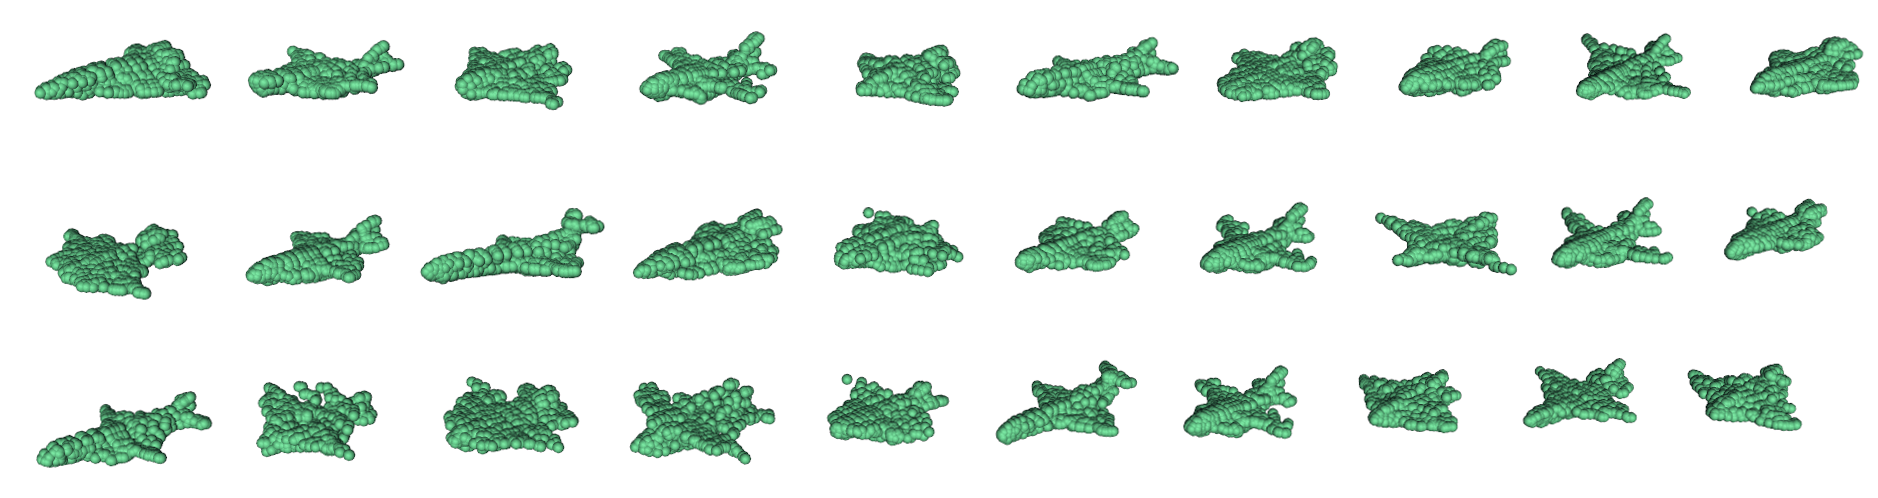
\includegraphics[width=1.0\linewidth]{PCAGAN/images/gallery/airplanes.png}

\includegraphics[width=1.0\linewidth]{PCAGAN/images/hline.png}
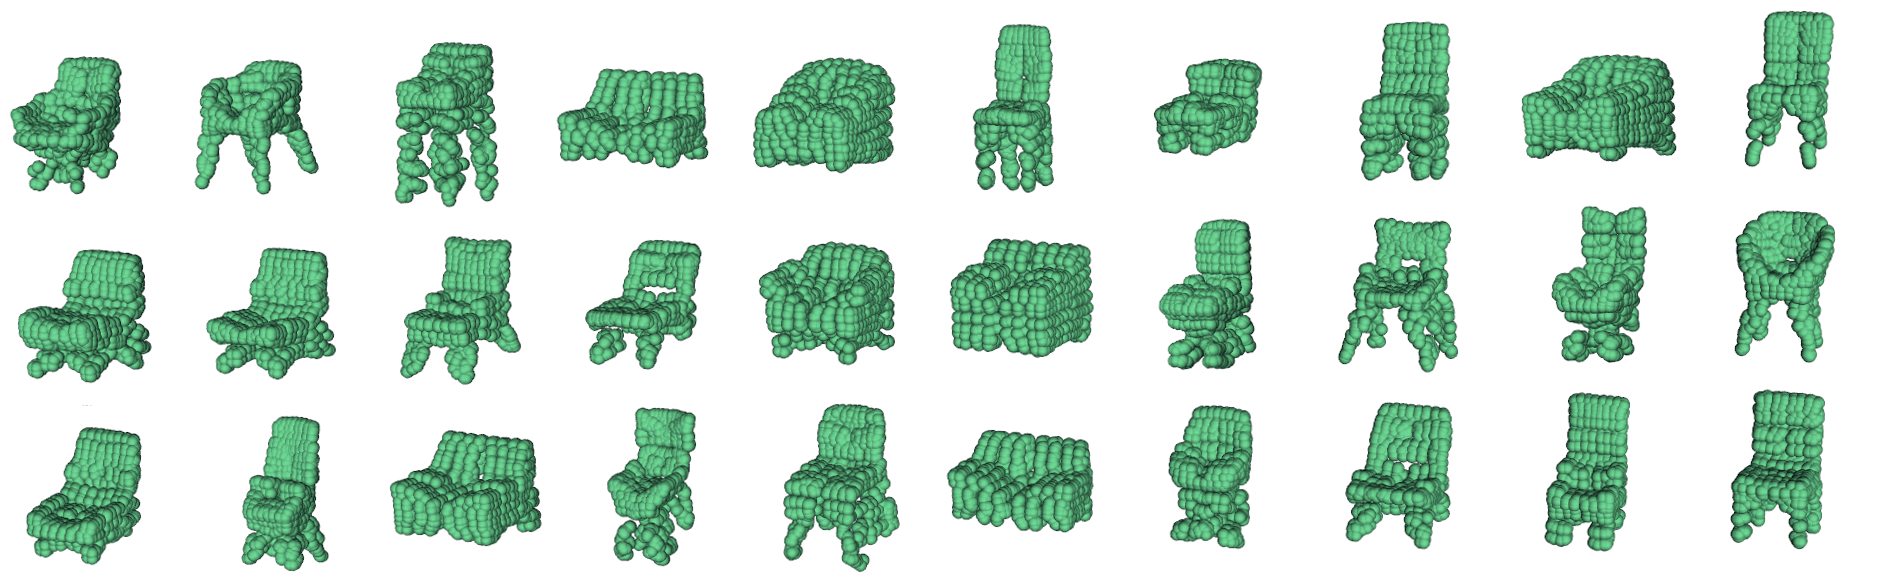
\includegraphics[width=1.0\linewidth]{PCAGAN/images/gallery/chairs.png}

\includegraphics[width=1.0\linewidth]{PCAGAN/images/hline.png}
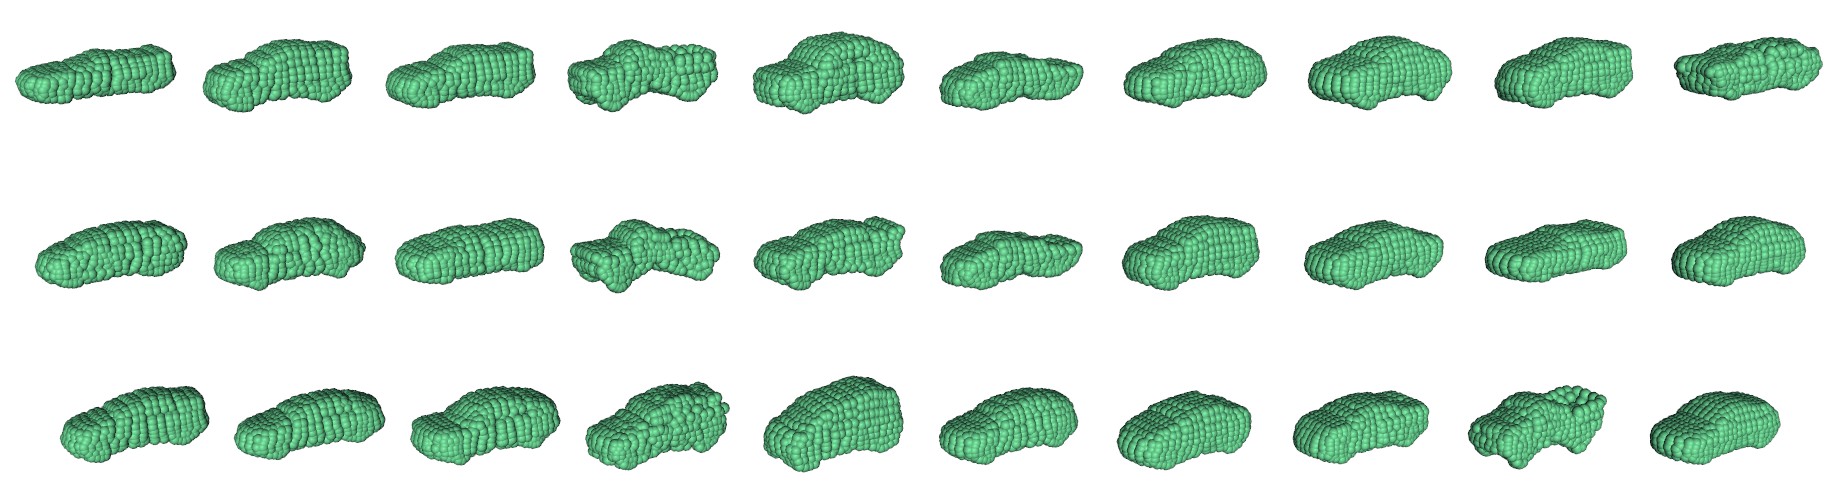
\includegraphics[width=1.0\linewidth]{PCAGAN/images/gallery/cars.png}
\vspace{-16pt}
\caption{\small \label{pca:gallery} A gallery showing results of using our method to generate points clouds for three categories: airplane, chair, and car. We use our method to train a GAN for each category separately. The training is generally very fast and completes within a few minutes. The results shown here are generated by randomly sampling the encoding $z$ of the GAN.}
\vspace{-12pt}
\end{figure}




\section{Experiments}\label{dmp:experiments}

\begin{table}[t]
\centering
\footnotesize
\tabcolsep=0.11cm
\begin{tabular}{|l|c|c|c||c|c|}
\hline
& Surface & Contour & Implicit & RIMLS\cite{rimls} & SPSR\cite{spsr} \\
\hline
bunny & \textbf{2.71E-04} & 6.64E-04 & 5.52E-04 & 1.43E-03 & 3.96E-04 \\
dragon & \textbf{4.18E-04} & 6.12E-04 & 1.20E-03 & 1.65E-03 & 1.46E-02 \\
car & \textbf{2.73E-04} & 4.57E-04 & 6.83E-02 & 1.50E-03 & 2.10E-03 \\
cup &  \textbf{2.59E-04} & 5.80E-04 & 2.64E-02 & 1.74E-03 & 1.00E-02 \\
mobius &  \textbf{3.51E-04} & 4.95E-04 & 3.26E-03 & 1.96E-03 & 1.89E-02 \\
chair &  \textbf{3.95E-04} & 4.22E-04 & 7.32E-03 & 2.09E-03 & 2.58E-02 \\
spiral &  1.05E-03 & \textbf{7.31E-04} & 1.64E-02 & 2.98E-03 & 7.90E-02 \\
ring &  5.69E-04 & \textbf{5.54E-04}& 4.81E-02 & 2.46E-03 & 3.76E-02 \\
\hline
avg. & \textbf{4.48E-04} & 5.65E-04& 2.13E-02 & 1.98E-03 & 2.36E-02 \\
\hline
\end{tabular}
\vspace{4pt}
\caption{ \small \label{tab:denoising} \textbf{Quantitative results for point cloud denoising.}
\emph{Surface}, \emph{Contour} and \emph{Implicit} represent different \emph{deep manifold priors} based on a 2-manifold, 1-manifold and level-set paramertization.
}
\vspace{-15pt}
\end{table}
\begin{table*}[t]
\centering
\scriptsize
\tabcolsep=0.11cm
\begin{tabular}{|l|c|c|c|c||c|c|}
\hline
& S1R & S8R & S1 & S8 & - & - \\
\hline
avg. & 4.48E-03 & \textbf{4.48E-04} & 2.75E-03 & 1.35E-03  & - & - \\
\hline \hline
& C1R & C8R & C1 & C8 & RIMLS\cite{rimls} & SPSR\cite{spsr} \\
\hline
avg. & 1.08E-03 & 5.77E-04 & 1.00E-03 & 5.82E-04 & 1.98E-03 & 2.36E-02 \\
\hline
\end{tabular}
\vspace{4pt}
\caption{ \small \label{tab:ablation} \textbf{Ablation studies.}
Comparison between different variations of our approach.
Naming follows the following convention: S corresponds to a 2-manifold parameterization (surface), whereas C corresponds to a 1-manifold (contour).
The following number (1 or 8) corresponds to the number of parameterizations.
A R letter is added if stretch regularization was used ($\lambda=1.0$).
}
\end{table*}

\begin{figure*}[t]
\centering
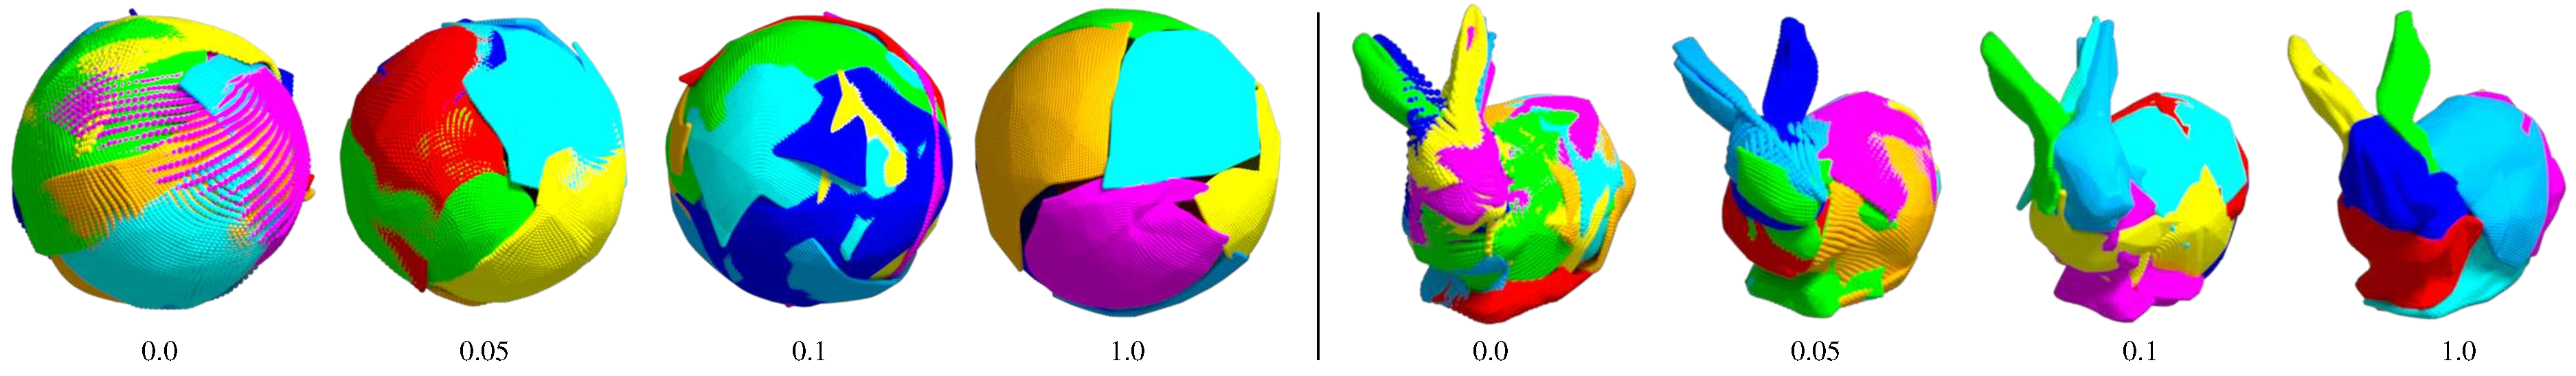
\includegraphics[width=\linewidth]{dmp/imgs/regularization.pdf}
	\caption{\label{fig:reg} \small
	\textbf{Effect of the regularization weight on the reconstructed manifold.} 
	For this experiment, we use our method to reconstruct a sphere using an atlas with 8 charts and render each one with a different color.
	Without any regularization, there is a significant amount of deformation applied to each surface (hence the space between the points) and a considerable amount of overlap between different parts. As the regularization weight increases, those aspects are
	noticeably reduced. 
	\small}
	\vspace{-12pt}
\end{figure*}

In this section we will present quantitative and qualitative results for
applying the manifold prior to multiple manifold reconstruction tasks.
All the experiments in this paper were implemented using Python 3.6 and PyTorch.
Computation was performed on TitanX GPUs. 

\subsection{Denoising and Interpolation}

\paragraph*{Benchmark} Our benchmark consists of 8 different 3D shapes with diverse characteristics.
The shapes are normalized to fit a unit cube and 16K points are sampled on their surfaces.
The point positions are perturbed by a Gaussian noise with standard deviation $2\times10^{-3}$ and zero mean.
Figure~\ref{fig:denoising} shows the ground-truth shapes as well
as their noisy counterpart.
Since the level-set representation and the baseline methods 
(RIMLS~\cite{rimls},  SPSR~\cite{spsr}) 
require normal information, we estimate the normal for every point by using the local frame defined by its nearest neighbors.
We experimented multiple numbers of neighbors for both baselines and used the value that led to the best results: 20 neighbors for SPSR and the level-set representation, 30 neighbors for RIMLS.
The network used in the level-set representation follows the same architecture
and training protocol
as the one used for the explicit parametrizations (described in the next paragraph).
However, it is trained to predict every point as outside (+1) or inside the surface (-1).
Points with positive values are generated by translating every point in the point cloud along the normal direction for a distance $\epsilon=2\times10^{-3}$.
Points with negative values are generated in the same way, but applying a displacement
to the opposite direction.
For RIMLS, we used a relative spatial filter size of 10, 15 projection iterations and a volumetric grid with $200^3$ resolution.
For SPSR, we used an octree with depth 7 and 8 iterations.

\paragraph*{Experimental setup}
Our method performs denoising by minimizing Equation~\ref{eq:objective}.
In this framework, $P$ is the noisy point cloud we are trying to reconstruct and $\bm{f_\theta}$ is a neural network.
In all experiments we use a neural network with 3 fully connected layers,
where the layers have 256, 128 and 64 hidden units, respectively.
The output of the networks is a point in $\mathbb{R}^3$.
The input can be either a point in $\mathbb{R}$ (1-manifold) or $\mathbb{R}^2$ (2-manifold).
We use $ReLU$ activations followed by batch normalization at each layer, except for the last, where we use a $tanh$ non-linearity.
We vary the architecture of $\bm{f_\theta}$ with respect to the number
of parameterizations (1 or 8) and dimensionality (1 or 2).
Additionally, we try each one of these architectural variations with
$\lambda=0$ and $\lambda=1.0$.
When using 8 parametrizations, 4096 points are sampled per parametrization.
When using just one parametrization, 16K points are sampled.
We optimize our objective through gradient descent using the Adam optimizer
with learning rate $10^{-3}$.
For evaluation, we uniformly sampled 16K points in the computed manifold (represented as a triangular mesh) and compute the Chamfer distance with respect to the ground-truth.

\paragraph*{Results and discussion.}
Our methods significantly outperform the baselines for most of the shapes.
Quantitative results can be seen in Table~\ref{tab:denoising} and the qualitative results are shown in Figure~\ref{fig:denoising}.
The numbers are computed using 8 parametrizations (for surfaces and curves) and
$\lambda=1.0$.
A comparison between different variations of our approach is displayed in Table~\ref{tab:ablation}.
RIMLS, SPSR and level-set representations (\emph{Implicit} in Table~\ref{tab:denoising}) 
have trouble reconstructing point clouds with a significant amount of noise.
This is due to the fact that those methods rely on accurate surface normal estimates to infer
inside/outside regions of the shape.
Besides, RIMLS and methods based on implicit functions (SPSR and level-set representations) work better when dealing with closed surfaces. 
Shapes that are better approximated by contours (ring, spiral, chair's legs) are particularly challenging for those approaches.
On the other hand, the networks parametrizing explicit functions (\emph{Surface} and \emph{Contour} in Table~\ref{tab:denoising}) are able to adapt to different structures and
present a fair performance across a diverse set of shapes.

The results in Table~\ref{tab:ablation} suggest that using multiple parametrizations gives a better approximation than just using a single one.
This happens because complex shapes are easier to represent by multiple parametrizations.
For example, while using a single 2-manifold parametrization, the ring tends to be approximated by a disk, which significantly increases the reconstruction error when
the points are uniformly sampled over the final mesh.
This behavior is illustrated in Figure~\ref{dmp:interp}.
Our ablation studies also indicate that using stretch regularization helps
parametrizations of both surfaces and contours.
Figure~\ref{fig:reg} shows the effect of stretch regularization for
two different shapes.
As the regularization weight increases, the overlap between different parameterizations becomes smaller.
When overlaps exist, the manifold representation is suboptimal --
the same regions are being generated multiple times.

\begin{figure}
\centering
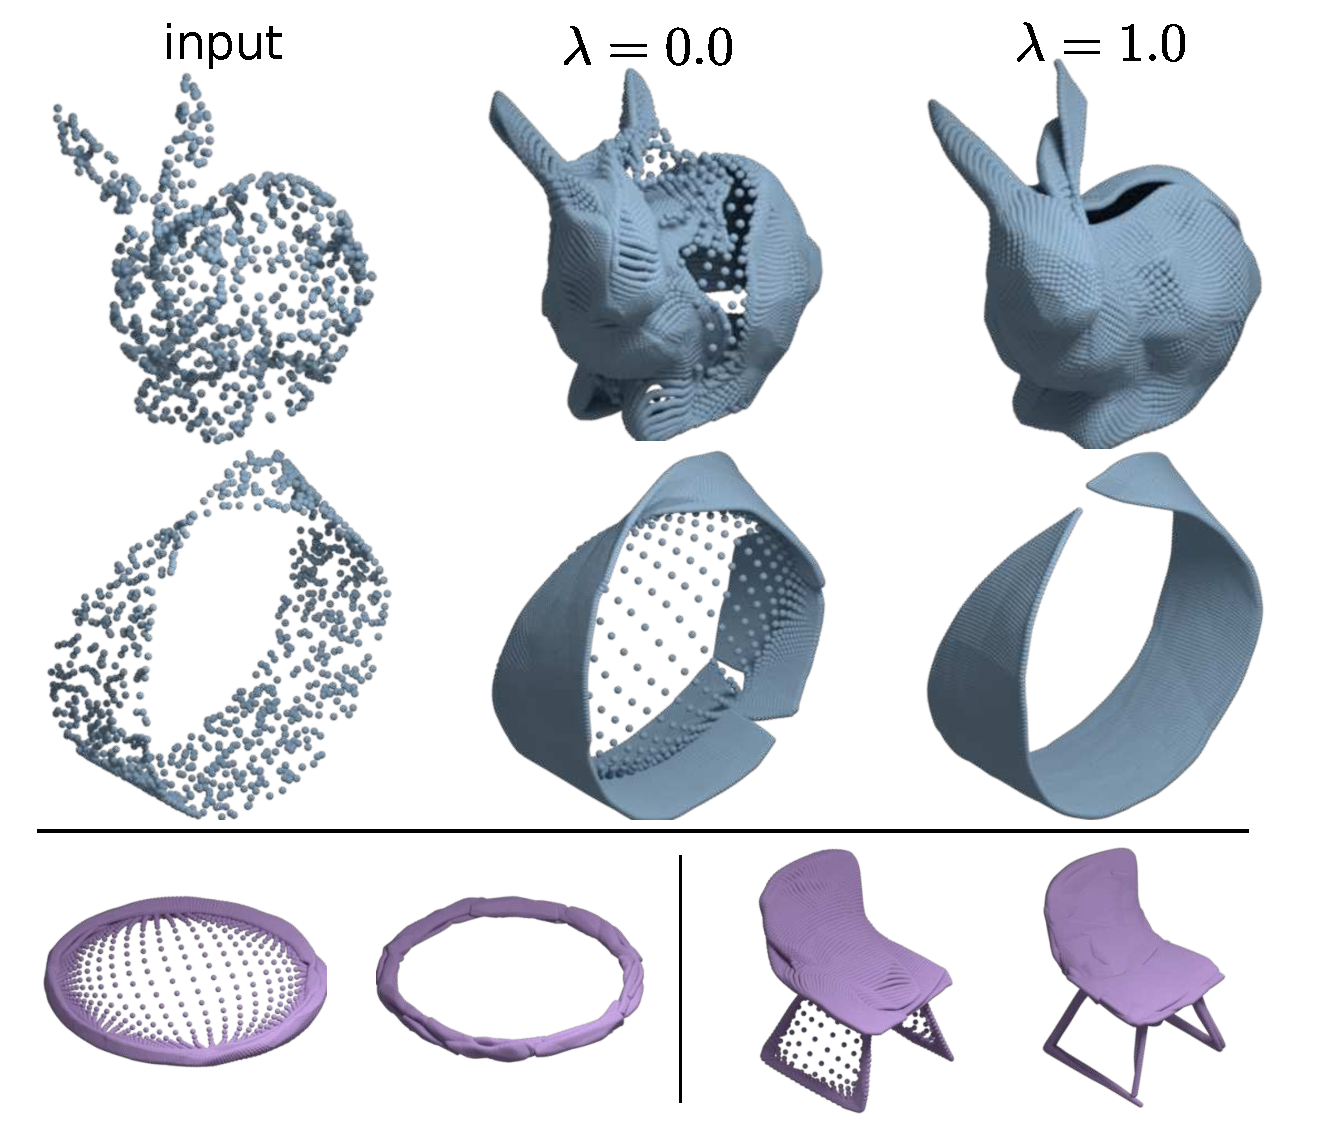
\includegraphics[width=0.6\linewidth]{dmp/imgs/interp_rings.pdf}
    \caption{\label{dmp:interp} \small 
    \emph{Interpolation results on the top.}
    Stretch regularization ($\lambda=1.0$) helps
    generate smoother surfaces.
    \emph{On the bottom, denoising using one vs. multiple parametrizations.}
   Shapes on the left were reconstructed using a single parameterization, 
    whereas shapes on the right used 8 parameterizations. 
    Using multiple parameterizations helps reconstruct complex shapes.
}
\vspace{-10pt}
\end{figure}


\begin{figure}[t!]
\centering
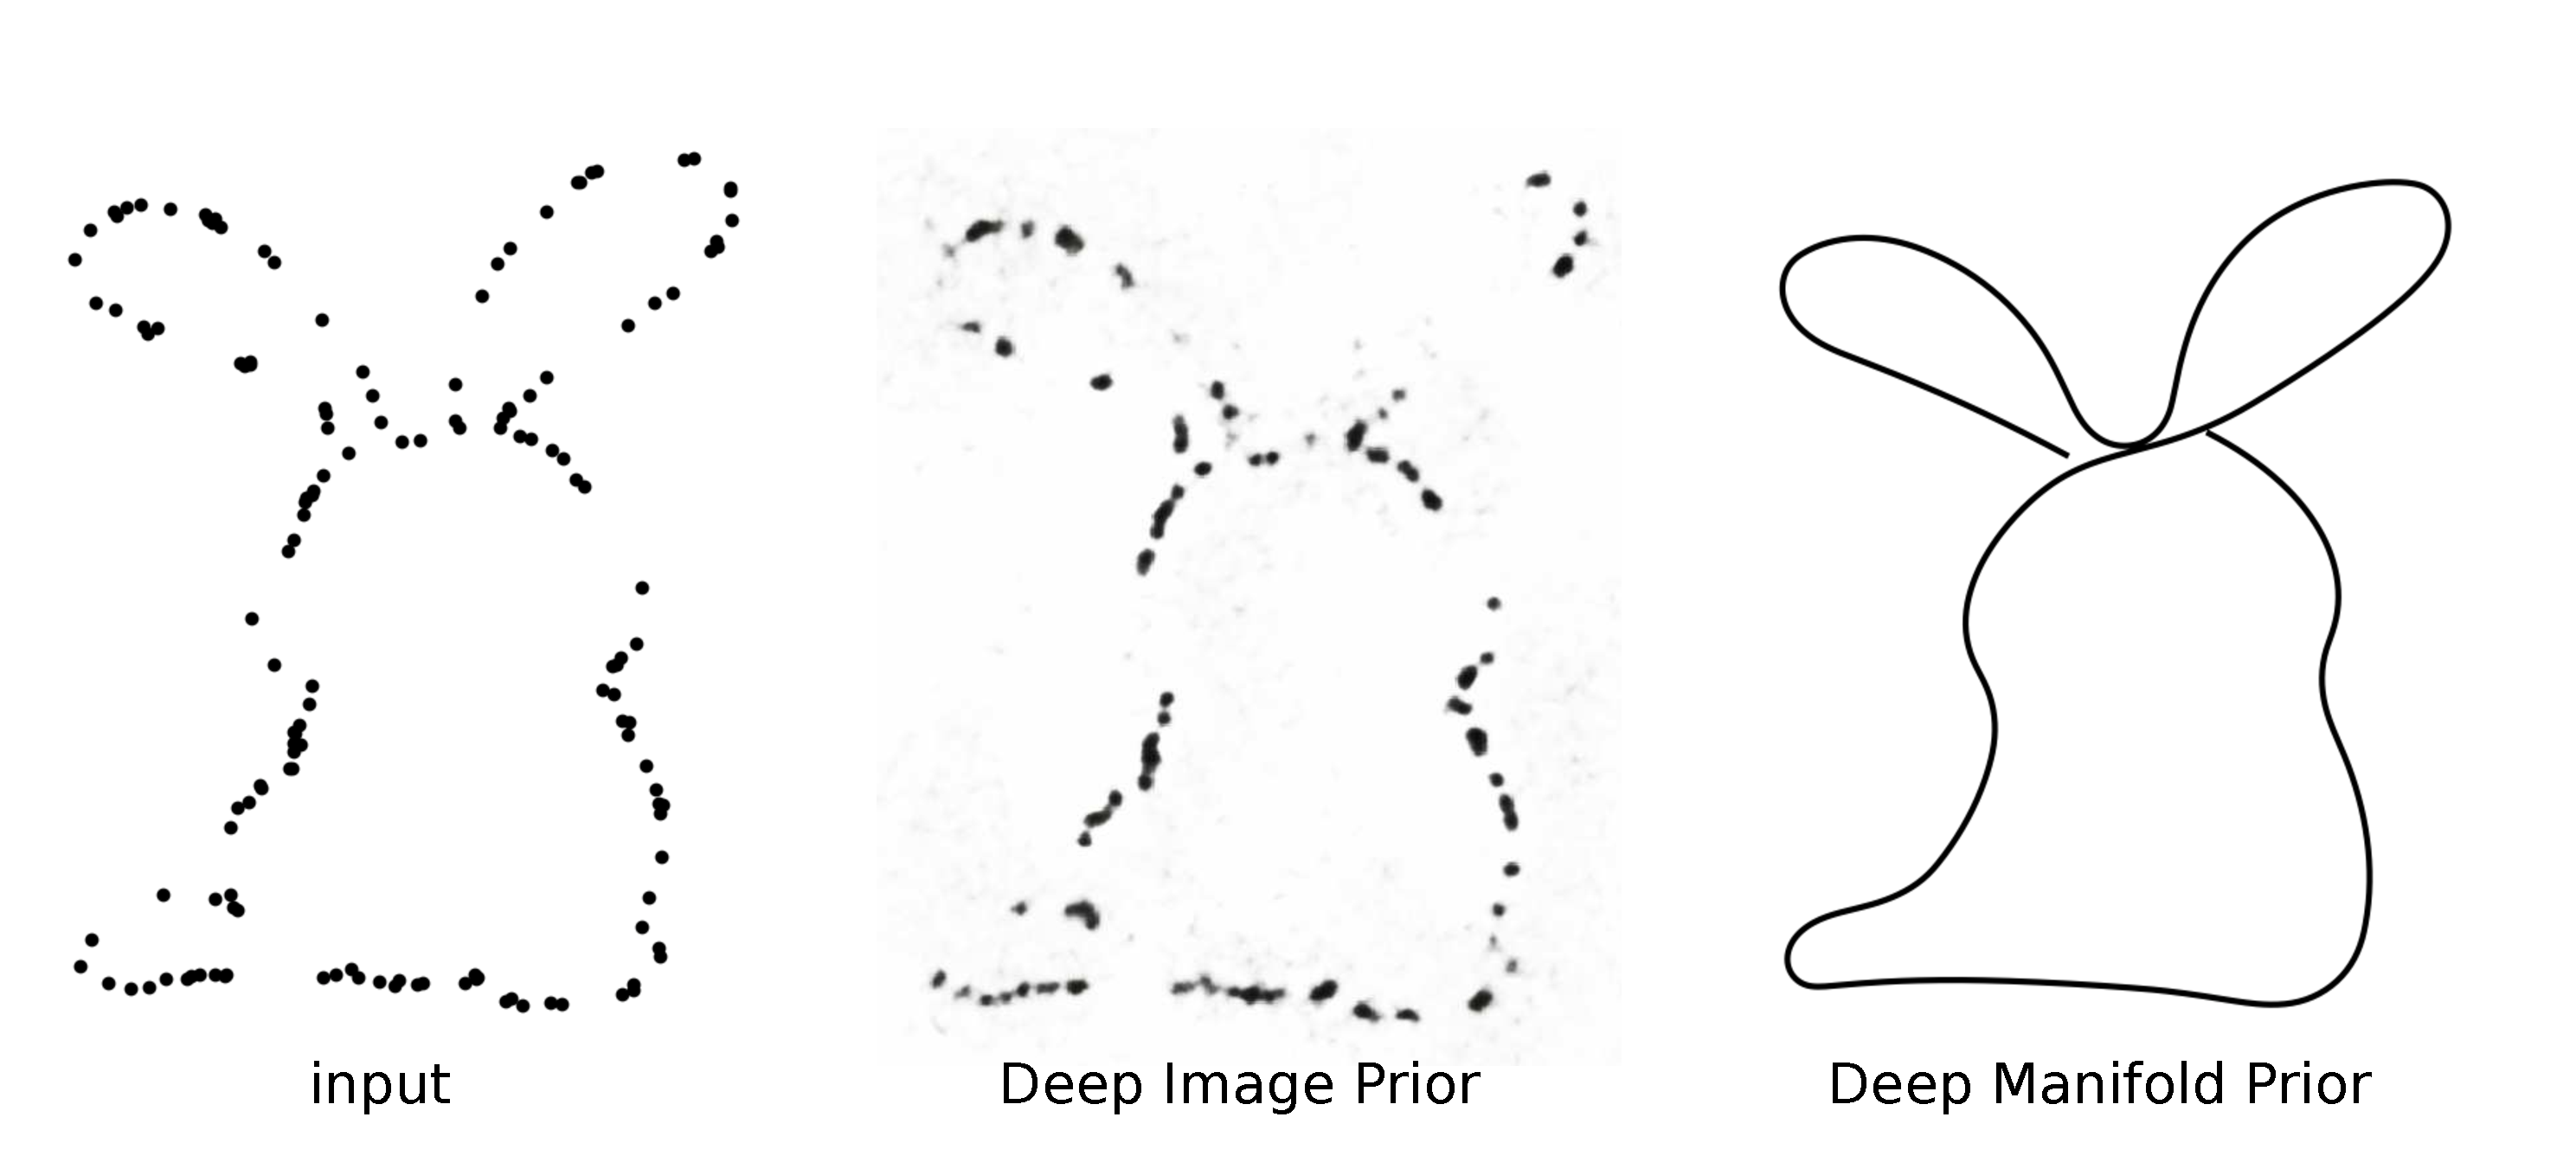
\includegraphics[width=0.8\linewidth]{dmp/imgs/dipcomp.pdf}
	\caption{\label{fig:dipcomp} \small
	\textbf{Comparison to the deep image prior~\cite{dip}.}
	Image-based prior (middle) is not able to connect the dots in the input image (left).
	On the other hand, the manifold prior is able to reasonably interpolate the dotted
	drawing.
	}
	\vspace{-18pt}
\end{figure}


\begin{figure*}[t]
\centering
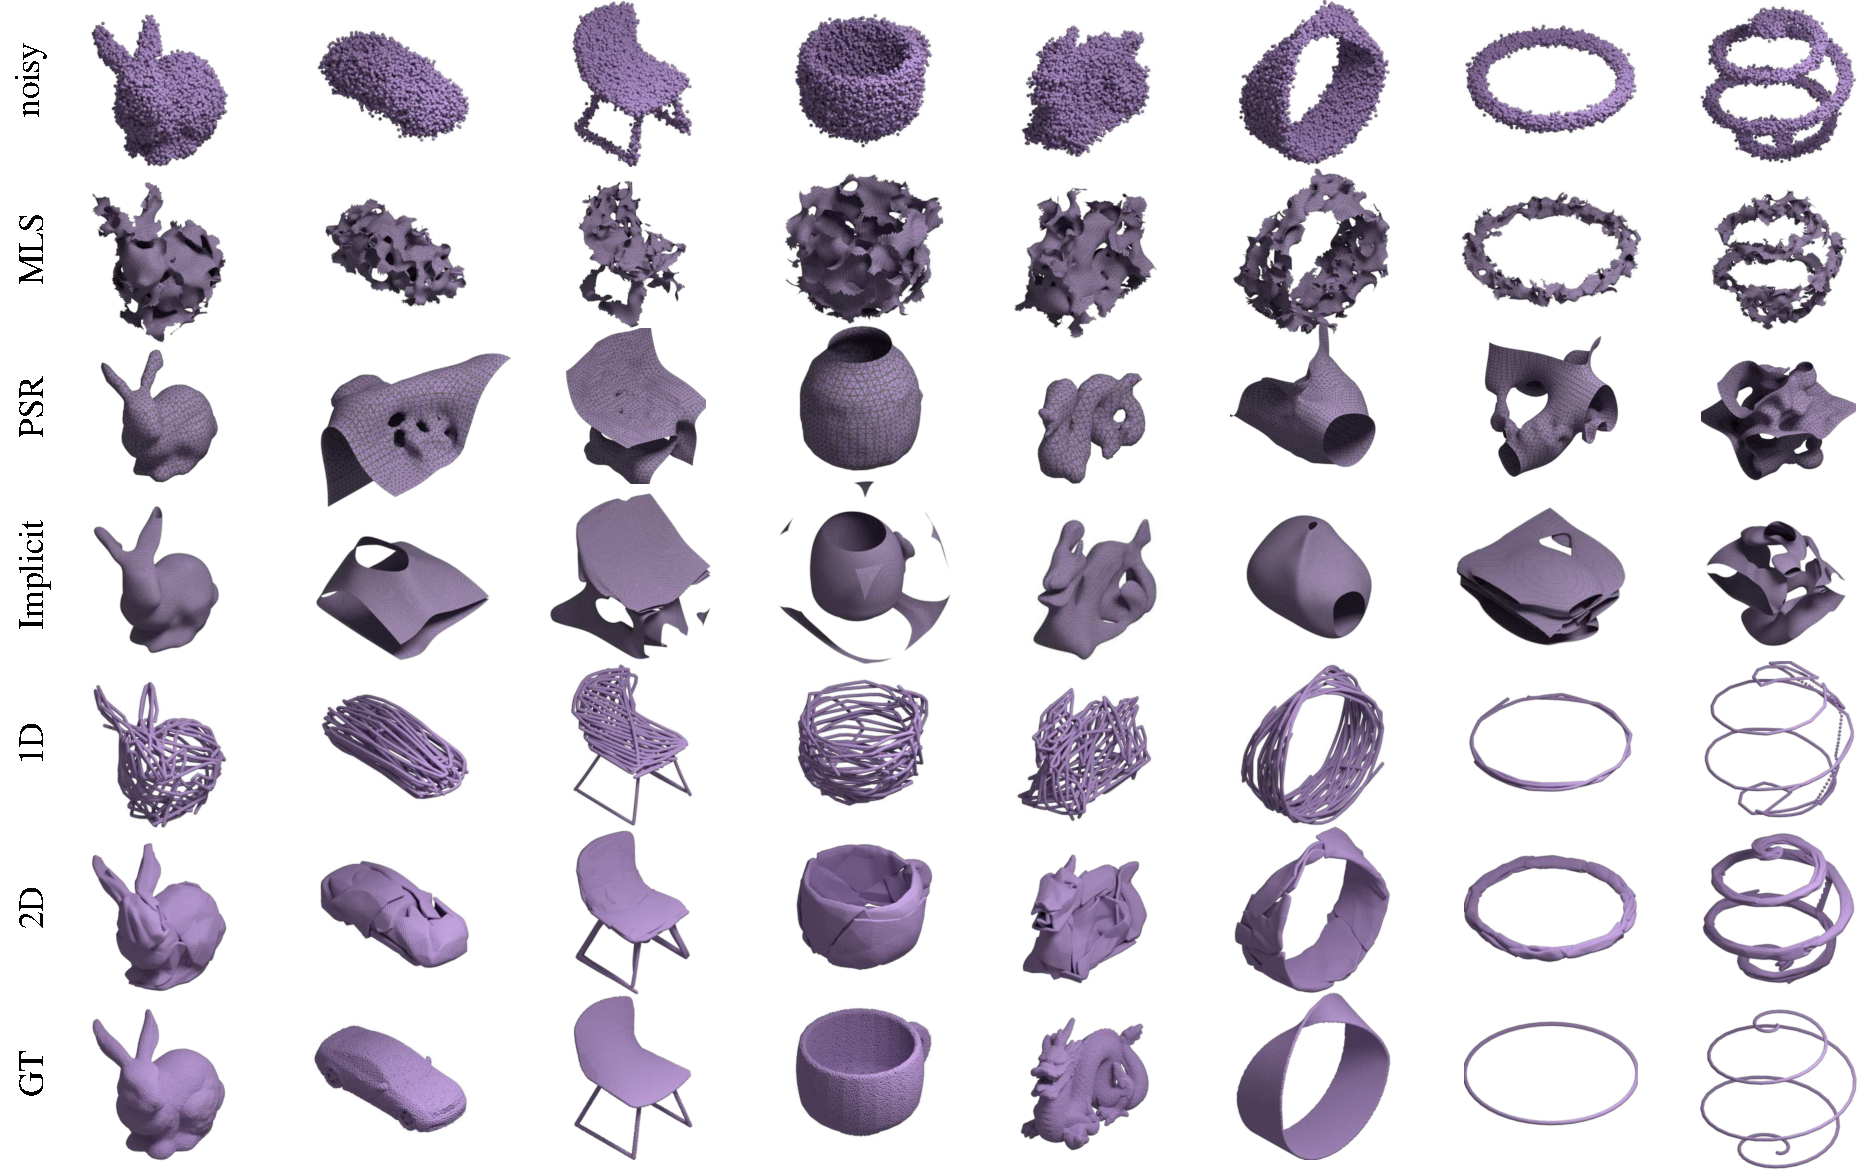
\includegraphics[width=1.0\linewidth]{dmp/imgs/denoising.pdf}
	\caption{\label{fig:denoising} \small
	\textbf{Qualitative comparison between different denoising methods.}
	Rows display different methods, whereas columns display different shapes.
	Baseline methods do not perform as well as the deep manifold prior, even for closed surfaces like the bunny (first column) and the dragon (fifth column).
	As we can see, 2-manifold parameterizations are better for reconstructing surfaces, whereas 1-manifold counterparts reconstruct the curves (last two columns) more
	acurattely.
	\small}
\end{figure*}

\paragraph*{Interpolation} We also explored using the manifold prior for point cloud interpolation.
This experiment follows the same experimental setup as denoising.
However, instead of perturbing the points with Gaussian noise, we randomly select 1K points out of 16K.
Interpolation is performed by minimizing Equation~\ref{eq:objective}.
Results can be seen in Figure~\ref{dmp:interp}.
For these experiments we use a single parameterization and include stretch regularization, without which the surface has holes and significant folds.
Our method is able to reconstruct reasonable surfaces from a small
set of points.

\paragraph*{Comparison with the deep image prior}
We also compare our approach to the deep image prior~\cite{dip} for interpolating points in 2D
images.
Results are presented in Figure~\ref{fig:dipcomp}.
We use the same architecture from \cite{dip} while minimizing
the mean squared error with respect to the image pixels.
For the manifold prior, we use a single 1-manifold parameterization following
the architecture described before, differing only in the dimensionality of the output: points this this case are in $\mathbb{R}^2$ instead of $\mathbb{R}^3$.
Coordinates of the black pixels in the input image are used to form a point cloud and 
the manifold is computed by minimizing Chamfer distance with respect to it.

\begin{figure}
\centering
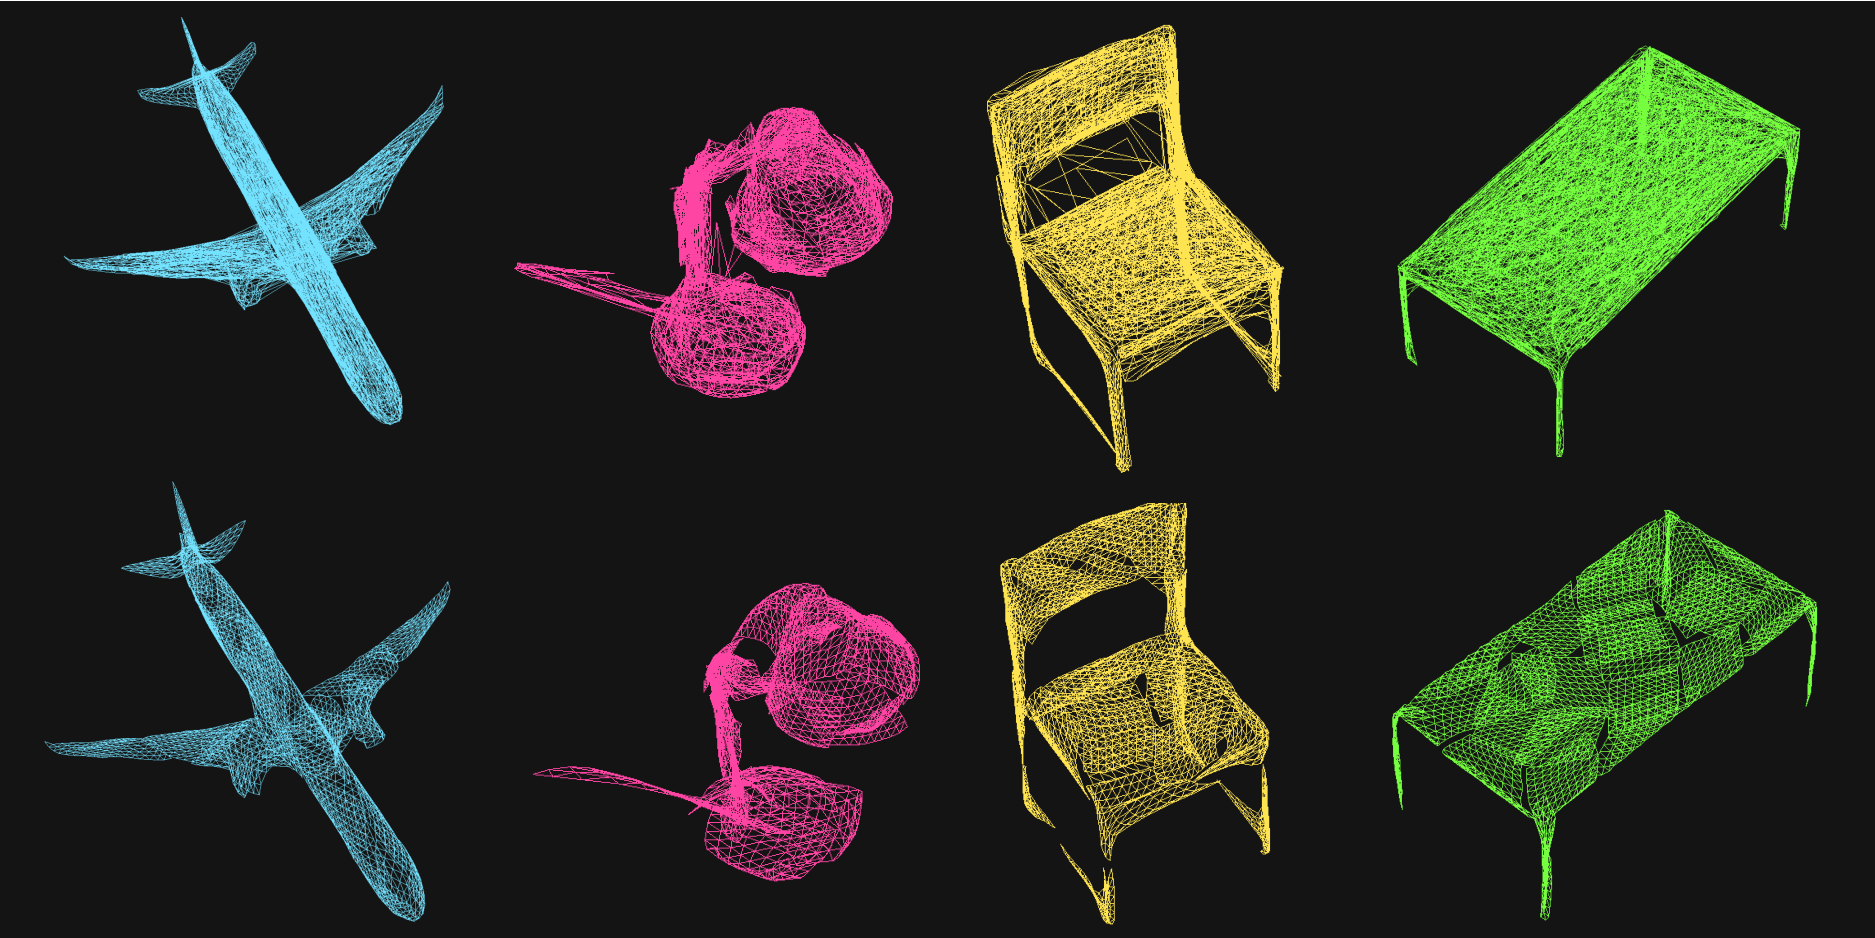
\includegraphics[width=0.8\linewidth]{dmp/imgs/aestretch.pdf}
    \caption{\label{fig:aestretch} \small \textbf{Autoencoder results}.
    Results on using AtlasNet~\cite{atlasnet} trained w/o (top) and w/ (bottom) stretch regularization.
    The latter results in meshes with reduced deformation and overlap, and removes artifacts where the chair's back is incorrectly filled.
}
\end{figure}

\subsection{Learning from data}\label{sec:exp_data}
Finally, we show how the insights presented in the earlier sections, in particular convolutional parameterization and stretch regularization, can also improve generative models of 3D shapes when trained on a large collection of shapes. 

To measure the effect of the stretch regularization in a learning-based scenario,
we train a model using the same architecture as AtlasNet~\cite{atlasnet} on a subset of $50,000$ shapes across $13$ categories of the ShapeNet dataset~\cite{chang2015shapenet}.
Adding stretch regularization did not significantly impact the Chamfer metric -- error of $1.46 \times 10^{-3}$ and $1.47 \times 10^{-3}$ with and without regularization.
However, the results are qualitatively better. 
As seen in Figure~\ref{fig:aestretch} the regularization reduces the stretch and overlap of the generated surfaces, and eliminates artifacts where holes are incorrectly filled.

We also train a convolutional decoder with stretch regularization on the single-view reconstruction benchmark~\cite{choy20163d}.
Our approach called ConvAtlas is compared against AtlasNet and MRTNet~\cite{mrt18} in Table~\ref{tab:svr}.
For a fair comparison, we use 4K points for evaluation across all methods.
ConvAtlas outperforms both approaches in terms of per-category and per-instance error, and also leads to more compact models.
Per-category results and experimental details are in the Supplementary material.


\begin{table}[t!]
\tabcolsep=0.11cm
\centering
\small
\begin{tabular}{|l|c|c|c|}
    \hline
    Architecture &  mean/cat. & mean/inst. & \#params. \\
    \hline
    MRTNet & 4.80 & 4.26 & 81.6M\\
    AtlasNet & 4.74 & 4.38 & 42.6M\\
    ConvAtlas & \textbf{4.53} & \textbf{4.00} & \textbf{ 14.5M}\\
    \hline
\end{tabular}
\vspace{4pt}
\caption{\small \textbf{Quantitative results for single-view image-to-shape reconstruction.} The table reports the mean Chamfer distance metric (scaled by $10^3$) computed per category and per instance.
  }
  \label{tab:svr}
  \vspace{-12pt}
\end{table}

\section{Discussion}

\section{Conclusion}
We presented a method to generate shapes represented as
sets of handles -- lightweight proxies that approximate the original
shape and are amenable to high-level tasks, like shape editing, parsing and animation.
Our approach leverages pre-defined sets of handles as supervision, either through annotated data or self-supervised methods. 
We proposed a versatile similarity metric for shape handles that can easily accommodate different types of handles, and a two-branch network architecture to generate handles with varying cardinality.
Experiments show that our model is capable of generating compact and accurate
shape approximations, outperforming previous work. We demonstrate our method in a variety of applications, including interactive shape editing, completion, and interpolation, leveraging the latent space learned by our model to guide these tasks.
\input{ack.tex}

\bibliographystyle{ieee_fullname}
\bibliography{egbib}

\end{document}
